\documentclass[letterpaper]{article} % DO NOT CHANGE THIS
\usepackage[submission]{aaai2027}  % DO NOT CHANGE THIS
% The serif, sans-serif, and monospaced fonts are loaded automatically by
% aaai2027.sty (newtxtext, helvet, courier). DO NOT add \usepackage{times},
% \usepackage{helvet}, \usepackage{courier}, or any other font package.
\usepackage[hyphens]{url}  % DO NOT CHANGE THIS
\usepackage{graphicx} % DO NOT CHANGE THIS
\urlstyle{rm} % DO NOT CHANGE THIS
\def\UrlFont{\rm}  % DO NOT CHANGE THIS
\usepackage{natbib}  % DO NOT CHANGE THIS AND DO NOT ADD ANY OPTIONS TO IT
\usepackage{caption} % DO NOT CHANGE THIS AND DO NOT ADD ANY OPTIONS TO IT
\usepackage{amsmath}
\frenchspacing  % DO NOT CHANGE THIS
%
% These are recommended to typeset algorithms but not required. See the subsubsection on algorithms. Remove them if you don't have algorithms in your paper.
\usepackage{algorithm}
\usepackage{algorithmic}

%
% These are recommended to typeset listings but not required. See the subsubsection on listing. Remove this block if you don't have listings in your paper.
\usepackage{newfloat}
\usepackage{listings}
\DeclareCaptionStyle{ruled}{labelfont=normalfont,labelsep=colon,strut=off} % DO NOT CHANGE THIS
\lstset{%
	basicstyle={\footnotesize\ttfamily},% footnotesize acceptable for monospace
	numbers=left,numberstyle=\footnotesize,xleftmargin=2em,% show line numbers, remove this entire line if you don't want the numbers.
	aboveskip=0pt,belowskip=0pt,%
	showstringspaces=false,tabsize=2,breaklines=true}
\floatstyle{ruled}
\newfloat{listing}{tb}{lst}{}
\floatname{listing}{Listing}

%
% Recommended for better-looking tables
\usepackage{booktabs}

% Paper-specific notation.
\newcommand{\method}{\textsc{MixerLoop}}
\newcommand{\Rel}{\operatorname{Rel}}
\newcommand{\Loc}{\operatorname{Loc}}
\DeclareMathOperator{\erank}{erank}
\newcommand{\Aop}{\mathcal{A}}
\newcommand{\Fop}{\mathcal{F}}

%
% Keep the \pdfinfo as shown here. There's no need
% for you to add the /Title and /Author tags.
\pdfinfo{
/TemplateVersion (2027.1)
}

% DISALLOWED PACKAGES
% \usepackage{authblk} -- This package is specifically forbidden
% \usepackage{balance} -- This package is specifically forbidden
% \usepackage{CJK} -- This package is specifically forbidden
% \usepackage{float} -- This package is specifically forbidden
% \usepackage{flushend} -- This package is specifically forbidden
% \usepackage{fullpage} -- This package is specifically forbidden
% \usepackage{geometry} -- This package is specifically forbidden
% \usepackage{hyperref} -- This package is specifically forbidden
% \usepackage{navigator} -- This package is specifically forbidden
% (or any other package that embeds links such as navigator or hyperref)
% \usepackage{indentfirst} -- This package is specifically forbidden
% \usepackage{layout} -- This package is specifically forbidden
% \usepackage{multicol} -- This package is specifically forbidden
% \usepackage{nameref} -- This package is specifically forbidden
% \usepackage{savetrees} -- This package is specifically forbidden
% \usepackage{setspace} -- This package is specifically forbidden
% \usepackage{stfloats} -- This package is specifically forbidden
% \usepackage{tabu} -- This package is specifically forbidden
% \usepackage{titlesec} -- This package is specifically forbidden
% \usepackage{tocbibind} -- This package is specifically forbidden
% \usepackage{ulem} -- This package is specifically forbidden
% \usepackage{wrapfig} -- This package is specifically forbidden
% DISALLOWED COMMANDS
% \nocopyright -- Your paper will not be published if you use this command
% \addtolength -- This command may not be used
% \balance -- This command may not be used
% \baselinestretch -- Your paper will not be published if you use this command
% \clearpage -- No page breaks of any kind may be used for the final version of your paper
% \columnsep -- This command may not be used
% \newpage -- No page breaks of any kind may be used for the final version of your paper
% \pagebreak -- No page breaks of any kind may be used for the final version of your paper
% \pagestyle -- This command may not be used
% \tiny -- This is not an acceptable font size.
% \vspace{- -- No negative value may be used in proximity of a caption, figure, table, section, subsection, subsubsection, or reference
% \vskip{- -- No negative value may be used to alter spacing above or below a caption, figure, table, section, subsection, subsubsection, or reference

\setcounter{secnumdepth}{0} %May be changed to 1 or 2 if section numbers are desired.

% The file aaai2027.sty is the style file for AAAI Press
% proceedings, working notes, and technical reports.
%

% Title

% Your title must be in mixed case, not sentence case.
% That means all verbs (including short verbs like be, is, using,and go),
% nouns, adverbs, adjectives should be capitalized, including both words in hyphenated terms, while
% articles, conjunctions, and prepositions are lower case unless they
% directly follow a colon or long dash
\title{Allocating Recurrent Compute in Looped Language Models}
\author{
    %Authors
    % All authors must be in the same font size and format.
    Ruhai Lin\textsuperscript{\rm 1}\equalcontrib,
    Yiyang Guo\textsuperscript{\rm 1}\equalcontrib,
    Rui-jie Zhu\textsuperscript{\rm 1},
    Hao Ye\textsuperscript{\rm 1},
    Jason Eshraghian\textsuperscript{\rm 1}\corresponding
}
\affiliations{
    %Afiliations
    \textsuperscript{\rm 1}University of California, Santa Cruz\\
    % If you have multiple authors and multiple affiliations
    % use superscripts in text and roman font to identify them.
    % For example,

    % Sunil Issar\textsuperscript{\rm 2},
    % J. Scott Penberthy\textsuperscript{\rm 3},
    % George Ferguson\textsuperscript{\rm 4}\corresponding,
    % Hans Guesgen\textsuperscript{\rm 5}
    % Note that the comma should be placed after the superscript

    1156 High St,\\
    Santa Cruz, CA 95064 USA\\
    % email address must be in roman text type, not monospace or sans serif
    rlin50@ucsc.edu
%
% See more examples next
}

%Example, Single Author, ->> remove \iffalse,\fi and place them surrounding AAAI title to use it
\iffalse
\title{My Publication Title --- Single Author}
\author {
    Author Name
}
\affiliations{
    Affiliation\\
    Affiliation Line 2\\
    name@example.com
}
\fi

\iffalse
%Example, Multiple Authors, ->> remove \iffalse,\fi and place them surrounding AAAI title to use it
\title{}
\author {
    % Authors
    Ruhai Lin\textsuperscript{\rm 1,\rm 2}\equalcontrib,
    Second Author Name\textsuperscript{\rm 2}\equalcontrib,
    Jason Eshraghian\textsuperscript{\rm 1}\corresponding
}
\affiliations {
    % Affiliations
    \textsuperscript{\rm 1}Affiliation 1\\
    \textsuperscript{\rm 2}Affiliation 2\\
    firstAuthor@affiliation1.com, secondAuthor@affilation2.com, thirdAuthor@affiliation1.com
}
\fi


\begin{document}
\raggedbottom

\maketitle

\begin{abstract}
    Looped language models improve reasoning and knowledge manipulation by applying shared computation repeatedly. Existing systems usually repeat an entire layer stack, although a mixer and a dense feed-forward network (FFN) perform different operations and have different costs. We ask a narrower question: \emph{what should loop?} We view recurrence as repeated composition of a state update and argue that an application is valuable when it exposes a new cross-position influence direction that remains observable at the task readout. Iterative Transport Rank (ITR) describes the cumulative influence trajectory; marginal ITR describes the nonredundant influence contributed by successive applications. This view motivates \method{}, which repeats each Gated DeltaNet mixer while applying its dense FFN once. We compare \method{} with no recurrence and full-block recurrence at 15M and 110M parameters under the same data, initialization, and architecture. A finite context-off intervention tests whether later mixer applications produce distinct, non-negligible, and beneficial changes at the final language-model readout. \method{} surpasses FullLoop on aggregate CORE at 15M and retains $41.5\%$ of its CORE improvement at 110M while reducing recurrent-backbone projection FLOPs by $45.9\%$. These results show that the benefits of recurrent depth can be retained without repeatedly executing the dense FFN.
\end{abstract}

% Uncomment the following to link to your code, datasets, an extended version or similar.
% You must keep this block between (not within) the abstract and the main body of the paper.
% Make sure that you do not de-anonymize yourself with these links.
% \begin{links}
%     \link{Code}{https://aaai.org/example/code}
%     \link{Datasets}{https://aaai.org/example/datasets}
%     \link{Extended version}{https://aaai.org/example/extended-version}
% \end{links}

\section{Introduction}

Weight-shared recurrence scales language-model computational depth without
adding unique parameters. Looped Transformers, from Universal Transformers to
recent models such as Ouro and LT2, repeatedly apply the same layers before the
final token prediction, letting fixed parameters perform multiple rounds of
latent computation. Most existing models still define recurrence at the block
level, repeating the token mixer and feed-forward network at every loop step.
This design shows that latent computation helps, but not which operator helps,
how to allocate recurrent compute within a block, or what makes an operator
worth repeating. SGT selectively loops high-entropy softmax attention heads
while applying the FFN once, but its criterion is tied to one-step
softmax-attention distributions and cannot explain LT2's gains from repeatedly
applying a stateful linear mixer. A general account of operator-selective
recurrence therefore remains missing: which component should receive additional
loop steps, and how can its marginal contribution be measured across recurrent
depth?

We address this question with \method{}, which separates recurrent token mixing
from repeated feed-forward computation. \method{} repeatedly applies the Gated
DeltaNet mixer while executing the dense FFN once, and is compared with matched
NoLoop and FullLoop baselines under the same unique parameter counts, token
budgets, data order, and optimization settings. To characterize successive
mixer applications, we introduce Iterative Transport Rank (ITR) and marginal
ITR, which measure cumulative and newly added cross-token influence diversity
across recurrent depth. A finite context-off intervention further tests whether
later mixer applications produce distinct, non-negligible, beneficial
final-readout changes. Across 15M and 110M models, mixer-only recurrence
consistently improves over NoLoop, surpasses FullLoop on aggregate CORE at 15M,
gives an intermediate capability--compute tradeoff at 110M, and reaches up to
$1.52\times$ FullLoop prefill throughput.

\begin{figure*}[t]
\centering
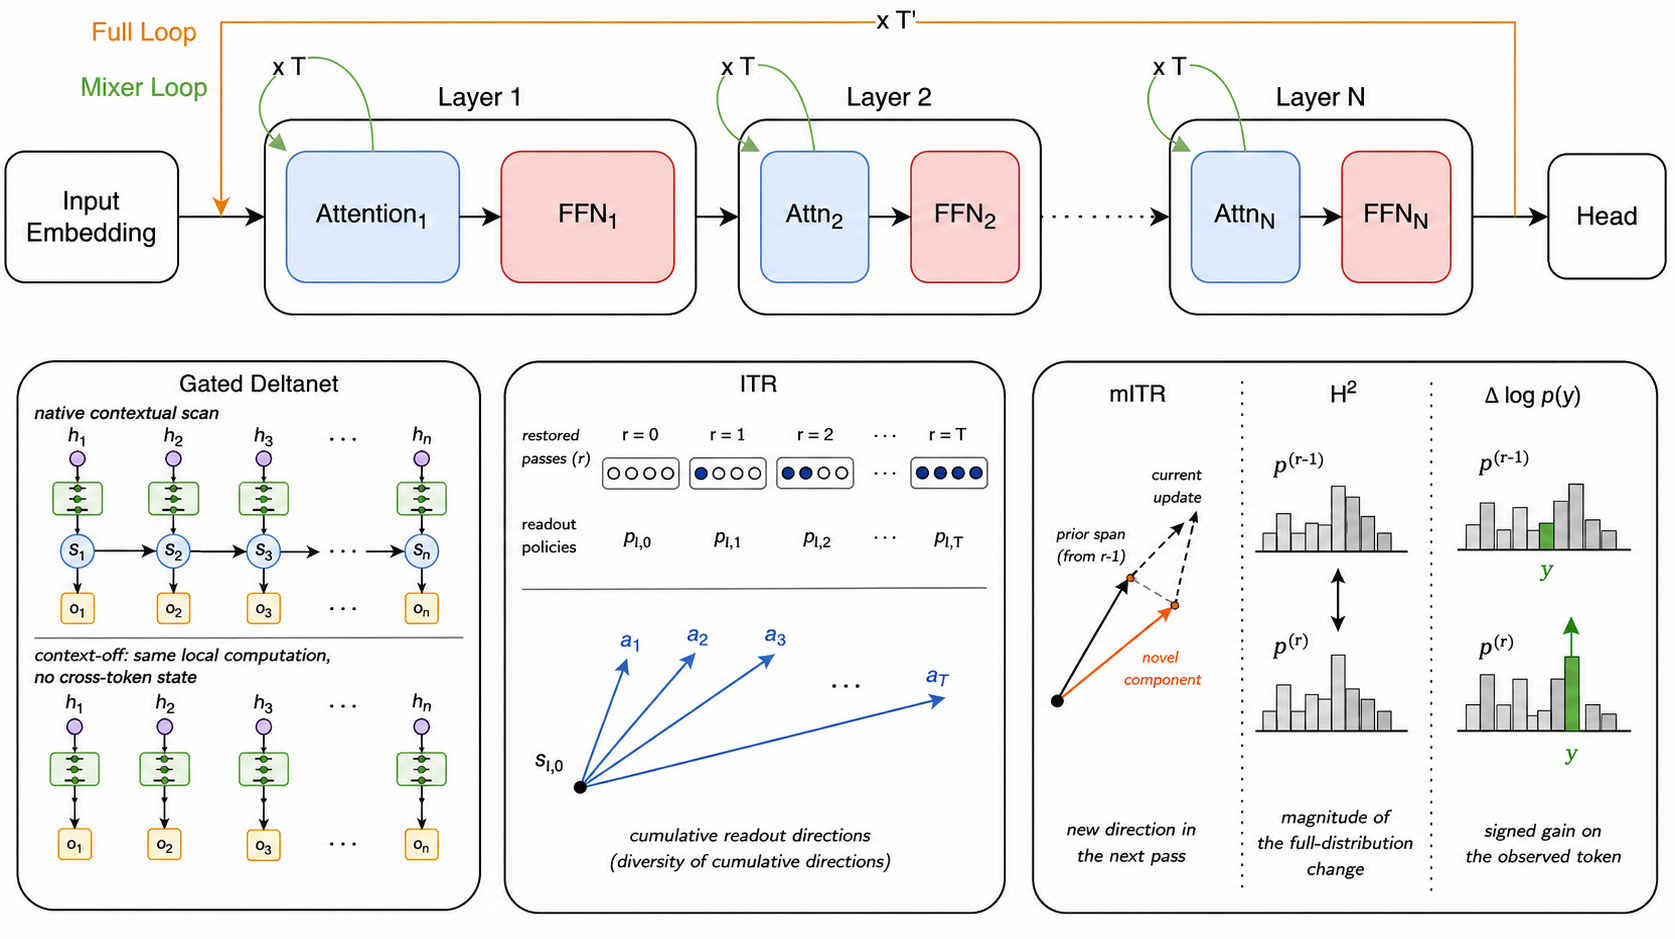
\includegraphics[width=0.96\textwidth]{Figures/main.png}
\caption{Overview of the motivation and architecture. A loop repeatedly
composes a state update, and useful applications expose cross-position effects
that remain observable at the final readout. \method{} repeats the shared GDN
mixer within each physical layer while applying the dense FFN once.}
\label{fig:overview}
\end{figure*}


\section{Related Work}

\paragraph{Looped Transformers and recurrent depth.}
Universal Transformers introduced depth-wise Transformer recurrence by
repeatedly applying a weight-shared block for fixed or adaptive steps
\cite{dehghani2019universaltransformers}. Subsequent work showed that this
inductive bias can improve systematic generalization and implement iterative
algorithms through repeated latent computation
\cite{yang2024loopedtransformersbetterlearning,saunshi2025reasoninglatentthoughtspower}.
This view now extends to language modeling at scale: Huginn adds a recurrent
core whose computation can increase at test time, Ouro repeatedly applies a
shared backbone and demonstrates favorable parameter scaling across
substantially larger training regimes, LT2 replaces quadratic attention with
linear and sparse token mixers, and MELT reduces recurrent-decoding memory
\cite{geiping2025scalingtesttimecomputelatent,zhu2025ouro,deng2026lt2lineartimeloopedtransformers,vendrell2026memoryefficient}.
Other models modify recurrent blocks with experts, attention mixtures,
polymorphic layers, or partial parameter specialization
\cite{csordas2024moeut,knupp2026depthrecurrentattentionmixturesgiving,chen2026polymorphicuniversal,zeitoun2026hyperlooptransformers}.
Additional methods allocate variable steps across tokens, layers, or compute
budgets, including SkipLayer, LoopFormer, Think-at-Hard, and
stability-regularized recurrence
\cite{li2025skiplayerloopit,jeddi2026loopformer,fu2026thinkhard,yang2026stabilizing,fan2025loopedtransformerslengthgeneralization}.
Together, these works expand when, where, and how long a model should recur.
Most retain the full Transformer block as the recurrent unit, leaving
within-block allocation unresolved.

\paragraph{Operator-selective recurrence.}
SGT is the closest precedent for recurrence below the block boundary. It
identifies high-entropy softmax attention heads, repeats them, and applies the
FFN once after recurrent attention \cite{chen2026sparsegrowingtransformertrainingtime}.
This shows that recurrent gains do not require every sublayer at every step,
but the entropy criterion does not extend directly to recurrent-state mixers.
Recurrent sparse FFNs are complementary: Sparse Layers and LoopMoE show
repeated FFN computation can remain useful when successive passes activate
different experts \cite{lee2026sparselayerscriticalscaling,chen2026loopmoeunifyingiterativecomputation}.
Together, these results suggest that recurrence value depends on the computation
exposed by successive applications, not on a fixed operator identity. This
motivates our comparison of no-loop, mixer-only, and full-block recurrence, and
our choice of a mixer whose state transition can be followed across recurrent
depth.

\paragraph{Linear attention as recurrent memory.}
Linear recurrent models naturally fit this study because they replace the
growing attention map with a fixed-size state updated across the sequence. S4
established structured state-space layers for long-range sequence modeling, and
RetNet connected recurrent state updates with an attention-like parallel
representation \cite{gu2022efficientlymodelinglong,sun2023retentivenetworksuccessor}.
Mamba introduced the selective state-space layer, S6, whose input-dependent
dynamics determine what enters, persists in, or leaves the recurrent state
\cite{gu2024mambalineartimesequence}. A related line interprets linear
attention as fast-weight memory: each token writes a key--value association into
a compact matrix state that later tokens query without storing the full
attention history \cite{schlag2021lineartransformerssecretlyfast}. DeltaNet
uses a delta-rule update to correct existing associations before writing new
information, and Gated DeltaNet adds adaptive forgetting to control long-range
state evolution \cite{yang2025gateddeltanetworksimproving}. Gated DeltaNet-2
separates erase and write operations, independently controlling which previous
memory components are removed and which new value components are committed
\cite{hatamizadeh2026gateddeltanet2}. This progression, from structured
recurrence to input-selective and overwrite-aware memory, makes linear
attention particularly suitable for operator-level looping: successive
applications can refine writing, forgetting, and retrieval while preserving
linear sequence complexity. We use GDN as the recurrent mixer and test whether state refinement provides an effective recurrent boundary without repeatedly executing the dense FFN


\section{Method}

\subsection{MixerLoop Architecture}

We build MixerLoop on the Gated DeltaNet backbone and change the
boundary at which recurrent computation is applied. Let $\Aop_i$ and $\Fop_i$
denote the residual token mixer and dense feed-forward network in physical layer
$i$:
\begin{align}
\Aop_i(h)
&=
h+
\operatorname{GDN}_i\!\left(
\operatorname{Norm}_{A,i}(h)
\right),\\
\Fop_i(h)
&=
h+
\operatorname{FFN}_i\!\left(
\operatorname{Norm}_{F,i}(h)
\right).
\end{align}
A non-recurrent model applies the mixer and FFN of each physical layer once:
\begin{equation}
h^{\mathrm{NoLoop}}
=\left(
\Fop_L\circ\Aop_L\circ\cdots\circ
\Fop_1\circ\Aop_1
\right)(h^0).
\label{eq:noloop}
\end{equation}
Existing full-loop language models instead reuse the complete backbone for
$T$ recurrent steps:
\begin{equation}
h^{\mathrm{FullLoop}}
=\left(
\Fop_L\circ\Aop_L\circ\cdots\circ
\Fop_1\circ\Aop_1
\right)^T(h^0).
\label{eq:fullloop}
\end{equation}
The output of one backbone pass becomes the input to the next, and every
recurrent step therefore executes both the token mixers and the dense FFNs.

MixerLoop moves recurrence inside each physical layer and applies it only to
the GDN mixer:
\begin{equation}
h^{\mathrm{MixerLoop}}
=\left(\Fop_L\circ\Aop_L^T\right)\circ\cdots\circ
\left(\Fop_1\circ\Aop_1^T\right)(h^0).
\label{eq:mixerloop}
\end{equation}
The $T$ applications of $\Aop_i$ share parameters, while different physical layers retain distinct mixer and FFN weights. MixerLoop therefore increases the effective depth of token mixing without increasing the number of unique parameters or repeatedly executing the dense FFN. Although the same GDN parameters are reused, successive applications do not repeat an identical computation. Each application receives the hidden sequence produced by the preceding pass and recomputes its input-dependent keys, values, decay gates, and delta-rule updates. It consequently induces a new sequence of memory writes, erasures, and reads over the causal recurrent state. MixerLoop allows this stateful token-mixing process to be refined several times before the resulting representation is passed through the dense FFN.

\begin{table}[t]
\centering
\small
\setlength{\tabcolsep}{2pt}
\begin{tabular}{@{}llc@{}}
\toprule
Model & Computation & Applications $(A,F)$ \\
\midrule
NoLoop
&
$\Fop_L\!\circ\!\Aop_L\!\circ\!\cdots$
&
$(1,1)$
\\
MixerLoop
&
$(\Fop_L\!\circ\!\Aop_L^T)\!\circ\!\cdots$
&
$(T,1)$
\\
FullLoop
&
$(\Fop_L\!\circ\!\Aop_L\!\circ\!\cdots)^T$
&
$(T,T)$
\\
\bottomrule
\end{tabular}
\caption{Recurrent boundaries studied in this work. $\Aop$ denotes the GDN
token mixer and $\Fop$ denotes the dense FFN. All models use the same physical
backbone and differ only in the placement of recurrent computation.}
\label{tab:architecture}
\end{table}

\subsection{Training Settings}

We compare architectures with matched unique parameter counts, data,
processed-token budgets, optimization settings, GDN backbone, tokenizer, context length,
and corpus. The nominal 15M/110M configurations respectively have
15.7M/116.9M unique parameters, 6/12 layers, width 288/768, 4/12 GDN heads, and
FFN width 768/2,048; both recurrent architectures use $T=4$, matching the LT2
loop count.

Training uses a 32K SentencePiece tokenizer, context length 1,024, the same
170-shard ClimbMix subset (10.69B corpus tokens) \cite{diao2026nemotronclimb},
100,000 streamed updates (52.43B processed tokens/model), and global batch
512. We use AdamW with $(\beta_1,\beta_2)=(0.9,0.95)$, peak learning rate
$5\times10^{-4}$, 1,000 warmup updates then cosine decay, weight decay $0.1$,
gradient clipping $1.0$, identical seed and data order, and no
architecture-specific hyperparameter search.

We evaluate the 22-task CORE suite from DataComp-LM
\cite{li2025datacomplmsearchgenerationtraining}, center each task against its
random baseline, and report both the CORE average and fixed manipulation subset
because looped models tend to gain more on information manipulation than
knowledge storage. The architecture comparison changes only the recurrent
boundary while model family, unique parameters, data, processed tokens, and
evaluation stay fixed.

\subsection{Estimated Compute Reduction}

Let $C_A$ and $C_F$ denote the projection FLOPs of
one GDN mixer and one dense FFN in a physical layer, and let $C_H$ denote the
cost of the final language-model head. Ignoring the shared embedding lookup,
the projection cost of one forward pass is
\begin{align}
C_{\mathrm{NoLoop}}
&=
L(C_A+C_F)+C_H,\\
C_{\mathrm{MixerLoop}}
&=
L(TC_A+C_F)+C_H,\\
C_{\mathrm{FullLoop}}
&=
TL(C_A+C_F)+C_H.
\end{align}
Relative to NoLoop, MixerLoop adds $L(T-1)C_A$ projection FLOPs, whereas
FullLoop adds $L(T-1)(C_A+C_F)$.

Within the recurrent backbone, the relative projection cost is
\begin{equation}
\frac{
C_{\mathrm{MixerLoop}}-C_H
}{
C_{\mathrm{FullLoop}}-C_H
}
=
\frac{TC_A+C_F}{T(C_A+C_F)}.
\label{eq:backbone_cost}
\end{equation}
Because dense FFNs account for $61.2$--$61.3\%$ of per-layer projection FLOPs,
Equation~\ref{eq:backbone_cost} gives $0.541$ at $T=4$:
\begin{equation}
\frac{TC_A+C_F}{T(C_A+C_F)}
=0.541.
\end{equation}
Thus MixerLoop retains $54.1\%$ of FullLoop backbone projection FLOPs and
reduces them by $45.9\%$.

Because every architecture executes the LM head once, end-to-end savings fall
to $33.9\%$ for 15M and $43.0\%$ for 110M; the 32K vocabulary head is a larger
compute share at 15M, while recurrent backbone compute dominates at 110M.
Prefill latency and throughput are measured in Section~\ref{sec:experiments}.

\subsection{Finite Iterative Transport Rank}
\label{sec:finite_itr}

We next ask why later mixer applications remain useful after repeated FFN computation has been removed. A direct
comparison of hidden states is insufficient for this purpose. Intermediate
representations may change substantially even when those changes are removed
by later layers or have negligible effect on the model's prediction. We
therefore measure iterative transport through a finite intervention and observe
its effect at the final language-model readout.

For each physical layer $\ell$, we construct a \emph{context-off} counterpart
of its native GDN mixer. The native mixer processes the sequence jointly through
its causal convolution and recurrent matrix state. The context-off mixer
preserves the same input projections, gates, normalization, residual path, and
token-local nonlinear computation, but processes each token independently. Its
causal convolution history and recurrent state are reset between tokens. The
intervention therefore removes only cross-position computation from the
selected mixer while leaving its token-local computation intact.

Suppose layer $\ell$ contains $T$ mixer occurrences. We define a sequence of
policies indexed by $r\in\{0,\ldots,T\}$. Under policy $r$, the first $r$
occurrences use the native contextual mixer, while the remaining $T-r$
occurrences use the context-off counterpart. Every other mixer, FFN, and
downstream operation remains unchanged. In MixerLoop, these occurrences are
consecutive within the same physical layer. In FullLoop, they appear at the
same layer across successive global backbone passes.

Let
\begin{equation}
p_{\ell,r}(\cdot\mid x_{\leq t})
\label{eq:intervention_distribution}
\end{equation}
denote the final next-token distribution produced under policy $r$. Policy
$r=0$ removes all contextual mixing from layer $\ell$, while policy $r=T$
recovers the native model exactly. Increasing $r$ from zero to $T$ therefore
restores the contextual mixer passes in their execution order and traces how
their effects accumulate at the final prediction.

We represent each predictive distribution by its elementwise square root:
\begin{equation}
s_{\ell,r}(x,t)
=\sqrt{
p_{\ell,r}(\cdot\mid x_{\leq t})
}.
\label{eq:sqrt_probability}
\end{equation}
This representation places every intervention in the same vocabulary-level
coordinate system. Euclidean distance in this space is proportional to
Hellinger distance between predictive distributions, allowing finite changes
in the model output to be compared without choosing a hidden-state basis.

For each restored depth $r$, we concatenate the change from the context-off
baseline across evaluated layers, sequences, and prediction positions:
\begin{equation}
a_r
=\operatorname{vec}_{\ell,x,t}\!\left[
s_{\ell,r}(x,t)-s_{\ell,0}(x,t)
\right],
\qquad
r=1,\ldots,T.
\label{eq:readout_trajectory}
\end{equation}
The vectors $\{a_1,\ldots,a_T\}$ form the cumulative readout trajectory.
Because the intervention differs only in the contextual computation performed
by layer $\ell$, $a_r$ measures the finite cross-token effect that survives the
remaining network and remains visible in the final predictive distribution.

To measure the diversity of this cumulative trajectory, we normalize each
nonzero direction,
\begin{equation}
z_r=\frac{a_r}{\|a_r\|_2},
\end{equation}
and construct the Gram matrix
\begin{equation}
K_{rs}=z_r^\top z_s.
\end{equation}
We define the Iterative Transport Rank as the participation-ratio rank of this
matrix:
\begin{equation}
\operatorname{ITR}_T
=\frac{\operatorname{tr}(K)^2}
{\operatorname{tr}(K^2)}.
\label{eq:itr}
\end{equation}
ITR lies between one and $T$. A value near one indicates that restoring
successive contextual passes moves the final prediction along a largely shared
cumulative direction. A larger value indicates that recurrent depth exposes a
more diverse trajectory of contextual effects at the readout. ITR measures the
geometry accumulated across all restored passes; it does not by itself
determine how much one particular pass contributes.

We therefore separately measure the novelty introduced by each additional
mixer application. Let
\begin{equation}
d_r=a_r-a_{r-1},
\qquad
a_0=0,
\end{equation}
be the finite readout update caused by restoring pass $r$. Let
$\Pi_{r-1}$ denote the orthogonal projection onto the span of the preceding
updates,
\begin{equation}
\operatorname{span}\{d_1,\ldots,d_{r-1}\}.
\end{equation}
The marginal Iterative Transport Rank of pass $r$ is
\begin{equation}
\operatorname{mITR}_r
=\frac{\left\|d_r-\Pi_{r-1}d_r\right\|_2^2}
{\|d_r\|_2^2}.
\label{eq:mitr}
\end{equation}
We set $\operatorname{mITR}_1=1$ and
$\operatorname{mITR}_r=0$ when $d_r=0$. Marginal ITR lies in $[0,1]$ and
measures the fraction of the current prediction update that cannot be expressed
by the updates of earlier contextual passes. A value near zero indicates that
the new pass largely follows an existing readout direction, whereas a value
near one indicates a substantially nonredundant correction.

For the layer-wise analysis, we apply the same definitions before
concatenating over layers, using
\begin{equation}
a_{\ell,r}
=\operatorname{vec}_{x,t}\!\left[
s_{\ell,r}(x,t)-s_{\ell,0}(x,t)
\right].
\label{eq:layerwise_readout_trajectory}
\end{equation}

A geometrically new direction is not necessarily important. It may have
negligible magnitude, or it may move the prediction away from the observed
target. We therefore accompany ITR with two quantities that measure the size
and sign of each restored pass. For layer $\ell$, sequence $x$, and prediction
position $t$, the squared Hellinger effect is
\begin{equation}
H_{\ell,r}^2(x,t)
=\frac{1}{2}
\left\|s_{\ell,r}(x,t)-s_{\ell,r-1}(x,t)\right\|_2^2.
\label{eq:hellinger}
\end{equation}
This measures how strongly pass $r$ changes the complete next-token
distribution. Its contribution to the observed next token $y$ is
\begin{equation}
g_{\ell,r}(x,t)
=\log p_{\ell,r}(y\mid x_{\leq t})-
\log p_{\ell,r-1}(y\mid x_{\leq t}).
\label{eq:true_token_gain}
\end{equation}
A positive value indicates that restoring the contextual pass increases the
probability assigned to the ground-truth token.

The four measurements answer distinct questions. ITR characterizes the
cumulative trajectory produced by recurrent contextual mixing. Marginal ITR
asks whether the next pass introduces a readout update not already represented
by earlier passes. Squared Hellinger distance determines whether that update is
large enough to alter the predictive distribution, and the ground-truth
log-probability change determines whether it moves the prediction in a useful
direction. Together, they test whether later mixer applications produce
distinct, non-negligible, and beneficial effects that survive to the final
language-model output.




\section{Experiments}
\label{sec:experiments}

We evaluate MixerLoop on three axes: language-modeling/downstream gains from
recurrent mixing without repeated FFNs, end-to-end throughput from lower
projection FLOPs, and whether later mixer applications produce distinct,
non-negligible, beneficial readout changes.

\subsection{Evaluation}

We report held-out next-token negative log-likelihood (NLL) and downstream
performance on the fixed 22-task CORE suite derived from DataComp-LM
\cite{li2025datacomplmsearchgenerationtraining}. Each downstream score is
centered against its random baseline and multiplied by 100, and CORE is the
unweighted mean across all 22 tasks. We additionally report the fixed
manipulation-oriented half of the suite as a separate aggregate, following the
observation that looped models can behave differently on knowledge storage and
knowledge manipulation. Every architecture uses the same task examples,
ordering, and few-shot demonstrations. The reported results correspond to one
final checkpoint per architecture; individual task scores are shown in full
rather than treating evaluation examples as independent training replicates.

For iterative transport, we sample held-out ClimbMix windows and evaluate
prediction positions from the second half of each sequence. The 15M analysis
uses 16 windows, 16 positions per window, and all six physical layers. The 110M
analysis uses eight windows, eight positions per window, and all twelve layers.
Readout directions are concatenated across vocabulary coordinates with equal
weight assigned to each evaluated layer and sequence window. As an
implementation check, restoring all $T$ native contextual passes reproduces the
unmodified model exactly in every evaluated run. Reported Hellinger effects and
ground-truth log-probability changes are averaged uniformly over evaluated
layers, windows, and prediction positions.

\begin{table*}[t]
\centering
\footnotesize
\setlength{\tabcolsep}{2.3pt}
\caption{CORE after 52.43B ClimbMix tokens with $T=4$. Panels follow the fixed
evaluation split. Scores are chance-adjusted and multiplied by 100; CORE
averages 22 tasks, and Manip.\ averages the lower-panel 11. Bold marks the best
result within each scale.}
\label{tab:core_main}
\begin{tabular}{lrrrrrrrrrrrr}
\toprule
Model
& Hella-ZS & Jeop. & WikiQA & ARC-E & ARC-C
& COPA & CSQA & PIQA & OBQA & LAMB. & BoolQ & CORE \\
\midrule
\multicolumn{13}{l}{\textit{15M parameters / 52.43B processed tokens}} \\
No Loop
& 4.20 & 0.14 & \textbf{8.42} & 18.01 & -3.07
& -16.00 & 1.21 & 20.13 & 3.73 & 13.04 & -26.43 & 5.01 \\
Full Loop (LT2)
& \textbf{4.61} & 0.05 & 6.38 & \textbf{19.08} & \textbf{-2.62}
& \textbf{-8.00} & -0.12 & \textbf{20.78} & 4.80 & 14.67 & -24.01 & 5.52 \\
\method{}
& 4.07 & \textbf{0.19} & 1.56 & 16.67 & -3.98
& -16.00 & \textbf{2.13} & 19.48 & \textbf{5.87} & \textbf{15.02} & \textbf{-6.87} & \textbf{6.52} \\
\midrule
\multicolumn{13}{l}{\textit{110M parameters / 52.43B processed tokens}} \\
No Loop
& 19.62 & 1.32 & 31.48 & 39.11 & 3.41
& 2.00 & 0.70 & 37.65 & 10.67 & 30.60 & -19.75 & 14.16 \\
Full Loop (LT2)
& \textbf{24.48} & \textbf{2.79} & \textbf{38.15} & \textbf{45.06} & \textbf{7.74}
& \textbf{12.00} & \textbf{14.21} & \textbf{38.30} & \textbf{14.67} & \textbf{32.35} & -21.60 & \textbf{17.52} \\
\method{}
& 21.13 & 2.41 & 35.30 & 41.86 & 6.94
& 8.00 & 10.42 & 37.76 & 11.73 & 30.66 & \textbf{-12.10} & 15.56 \\
\bottomrule
\end{tabular}

\vspace{4pt}

\begin{tabular}{lrrrrrrrrrrrr}
\toprule
Model
& Hella. & Wino. & WinoG. & Dyck & LSAT-AR
& CS-Alg. & Oper. & Repeat & SQuAD & CoQA & Lang-ID & Manip. \\
\midrule
\multicolumn{13}{l}{\textit{15M parameters / 52.43B processed tokens}} \\
No Loop
& 3.39 & 0.37 & -1.82 & 1.10 & \textbf{7.07}
& \textbf{39.47} & \textbf{13.81} & \textbf{0.00} & 0.99 & 4.41 & 17.96 & 7.89 \\
Full Loop (LT2)
& \textbf{4.19} & 6.96 & -3.55 & 0.70 & 4.35
& 38.48 & 9.05 & \textbf{0.00} & \textbf{1.68} & \textbf{5.56} & \textbf{18.38} & 7.80 \\
\method{}
& 3.83 & \textbf{9.89} & \textbf{4.81} & \textbf{8.90} & 5.43
& 37.05 & 10.95 & \textbf{0.00} & 1.32 & 5.51 & 17.56 & \textbf{9.57} \\
\midrule
\multicolumn{13}{l}{\textit{110M parameters / 52.43B processed tokens}} \\
No Loop
& 18.89 & 12.09 & 4.18 & 15.00 & \textbf{8.70}
& \textbf{45.08} & 14.76 & 0.00 & 6.45 & 11.56 & 18.01 & 14.07 \\
Full Loop (LT2)
& \textbf{24.29} & \textbf{18.68} & \textbf{4.50} & \textbf{19.90} & 7.07
& 43.18 & \textbf{15.24} & \textbf{3.13} & \textbf{9.79} & \textbf{14.19} & 17.40 & \textbf{16.12} \\
\method{}
& 20.64 & 16.48 & 2.76 & 9.80 & 3.80
& 43.03 & 12.38 & 0.00 & 8.03 & 12.60 & \textbf{18.59} & 13.46 \\
\bottomrule
\end{tabular}
\end{table*}

\subsection{Language Modeling and Downstream Performance}

Table~\ref{tab:core_main} compares recurrent boundaries at matched parameter
and training-token budgets. At 15M, MixerLoop reaches CORE $6.52$, above
NoLoop's $5.01$ and FullLoop's $5.52$. It also has the strongest manipulation
aggregate, improving from $7.89$ with NoLoop to $9.57$, while FullLoop reaches
$7.80$. Thus, repeating the complete backbone gives no aggregate CORE or
manipulation advantage over MixerLoop at this scale.

At 110M, all models improve and full recurrence helps more. MixerLoop raises
CORE from $14.16$ to $15.56$, while FullLoop reaches $17.52$. Relative to
NoLoop, MixerLoop retains $41.5\%$ of the full-loop CORE improvement while
using only $54.1\%$ of its recurrent-backbone projection FLOPs. Its upper-panel
gains include HellaSwag zero-shot, Jeopardy, WikiQA, ARC, COPA, CSQA, PIQA, and
OpenBookQA. FullLoop remains stronger on the aggregate and several
manipulation tasks, especially Dyck, Repeat Copy Logic, SQuAD, and CoQA.
MixerLoop therefore achieves a stronger aggregate capability--compute tradeoff
than FullLoop at 15M.

Held-out NLL follows the same ordering: NoLoop/MixerLoop/FullLoop NLLs are
$2.995$/$2.946$/$2.936$ at 15M and $2.401$/$2.377$/$2.342$ at 110M. MixerLoop
improves over NoLoop, while FullLoop keeps a small NLL edge; however, NLL does
not uniformly predict downstream results, since 15M MixerLoop has the highest
CORE despite FullLoop's lower NLL.

\subsection{Inference Efficiency}

Projection analysis predicts that MixerLoop removes $45.9\%$ of recurrent
backbone projections; we test end-to-end impact with BF16 prefill at length
1,024 on one RTX 3090 Ti, returning only final-token logits after six warmup
forwards and 20 timed forwards.

At batch size one, MixerLoop is $1.12\times$ faster than FullLoop at 15M and
$1.11\times$ at 110M, below the projection-FLOP ratio because the language-model
head is unchanged and short recurrent kernels remain launch/scheduling
dominated; larger batches improve arithmetic utilization. At the largest
measured batches, median latency drops from FullLoop to MixerLoop: $62.1$ to
$46.4$ ms for 15M at batch 32 ($1.34\times$ throughput) and $236.3$ to $155.5$
ms for 110M at batch 16 ($1.52\times$). Removing repeated FFNs therefore yields
measurable wall-clock gains, largest when backbone computation dominates kernel
overhead.

\subsection{Iterative Transport at the Readout}

To explain the capability results, we apply the finite intervention from
Section~\ref{sec:finite_itr} one layer at a time: start context-off, restore
native contextual mixer passes in execution order, and measure cumulative ITR,
per-pass $H^2$, and $\Delta\log p(y)$ (Figure~\ref{fig:readout_itr}).

\begin{figure*}[t]
\centering
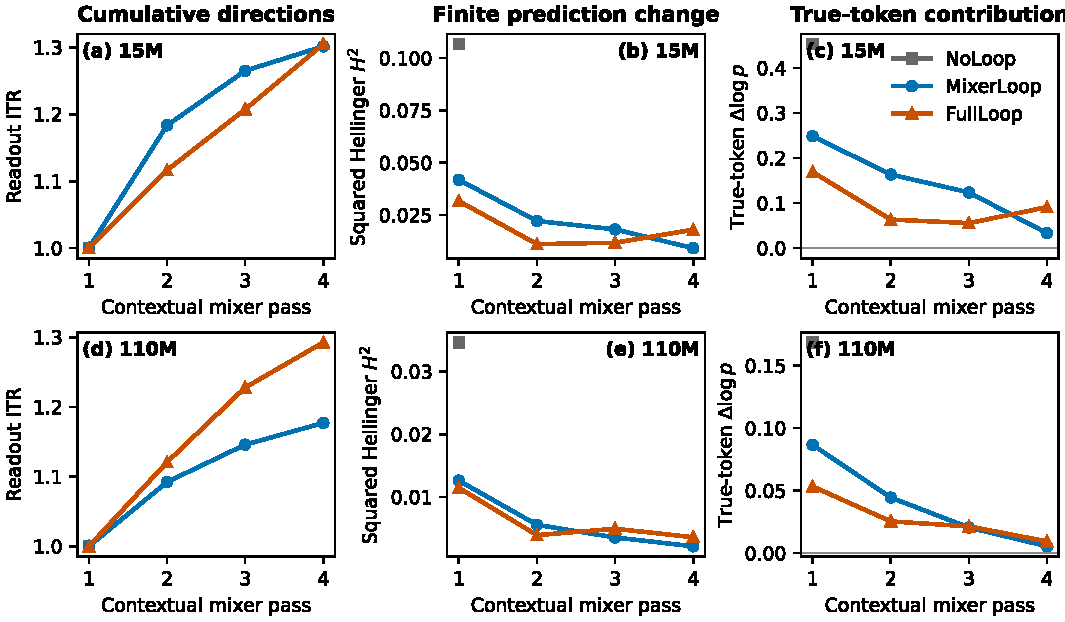
\includegraphics[width=0.82\textwidth]{Figures/readout_itr.pdf}
\caption{Finite iterative transport at 15M (top) and 110M (bottom). For each
physical layer, contextual mixer passes are restored in execution order. Left:
cumulative readout ITR. Middle: per-pass squared Hellinger effect. Right:
ground-truth next-token $\Delta\log p$. Middle/right values are uniformly
averaged over evaluated layers, held-out windows, and prediction positions.}
\label{fig:readout_itr}
\end{figure*}

At 15M, MixerLoop reaches ITR $1.301$ after four contextual passes, closely
matching FullLoop's $1.305$. Its marginal ITR values for passes two through four
are $0.988$, $0.871$, and $0.777$. The later applications therefore do not
merely extend the first pass along an unchanged readout direction. Together,
they account for $54.2\%$ of the sum of the per-pass squared Hellinger effects,
and each restored pass increases the probability of the observed next token.
Passes two through four contribute $+0.321$ nats in aggregate, compared with
$+0.210$ nats for FullLoop. At this scale, MixerLoop reaches essentially the
same cumulative transport diversity as FullLoop and produces a larger
beneficial correction from its later mixer applications.

The same qualitative result remains at 110M, although the trajectories separate
more clearly. MixerLoop reaches ITR $1.177$, with marginal ITR values of
$0.786$, $0.688$, and $0.672$ for its later passes. These applications account
for $47.2\%$ of the sum of the per-pass squared Hellinger effects and jointly
add $+0.070$ nats to the ground-truth log probability. FullLoop follows a more
diverse cumulative trajectory, reaching ITR $1.293$, but its later passes
contribute a slightly smaller signed gain of $+0.056$ nats. The comparison
illustrates why ITR is not itself a capability score: FullLoop can span a more
diverse predictive trajectory while MixerLoop's later corrections remain at
least as well aligned with the observed target.

These results provide a readout-level explanation for the architectural
comparison. Reusing the GDN mixer does not simply reproduce the contextual
effect of its first application. Later applications continue to generate
nonredundant changes in the final predictive distribution, and later passes
contribute a substantial share of the summed per-pass Hellinger effects.
Repeated FFN computation is therefore not required for the mixer to construct a
multi-step prediction trajectory.

\subsection{Controls and Layer-Wise Saturation}

A randomly initialized 15M MixerLoop model controls for the possibility that
marginal ITR reflects arbitrary high-dimensional variation. Its cumulative ITR
is only $1.068$, and its marginal ITR decreases to $0.440$, $0.283$, and
$0.241$ across the later passes. More importantly, the average squared
Hellinger effect of each pass is only $6.4\times10^{-6}$, and passes two through
four jointly change the target log probability by $-1.5\times10^{-4}$ nats.
Training therefore changes all three properties measured by the intervention:
the readout updates become more diverse, acquire non-negligible magnitude, and
become positively aligned with the observed next token.

The result is also stable to the intervention sample. On an independently
sampled set of held-out windows, the trained 15M ITR is $1.313$ for MixerLoop
and $1.284$ for FullLoop. Increasing the analyzed context length from 128 to
256 tokens gives corresponding values of $1.327$ and $1.311$. The exact values
vary slightly with the evaluation surface, but both recurrent architectures
continue to exhibit a multi-pass readout trajectory.

\begin{figure}[t]
\centering
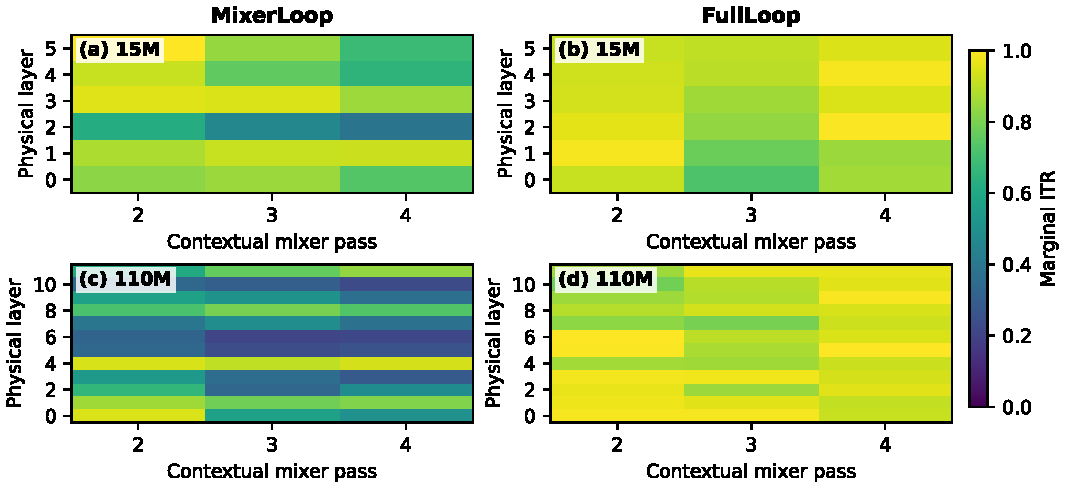
\includegraphics[width=\columnwidth]{Figures/layerwise_mitr.pdf}
\caption{Layer-wise marginal ITR for contextual passes two through four. Each
cell reports the fraction of a pass's finite readout update that lies outside
the span of earlier updates in the same physical layer. MixerLoop retains
broadly distributed novelty at 15M and a more selective pattern at 110M,
whereas FullLoop maintains high geometric novelty across the stack.}
\label{fig:layerwise_mitr}
\end{figure}

Figure~\ref{fig:layerwise_mitr} resolves the aggregate trajectory across
physical layers. At 15M, 16 of the 18 later MixerLoop layer--pass pairs have
marginal ITR above $0.5$, and all 18 have a positive mean ground-truth
log-probability contribution. Useful recurrent mixing is therefore distributed
across nearly the entire model rather than concentrated in one or two layers.
At 110M, 19 of 36 later layer--pass pairs remain above $0.5$, while 30 of 36
have a positive mean target contribution. Recurrent novelty becomes more
selective as the model scales, but most later mixer applications remain
beneficial.

FullLoop maintains marginal ITR above $0.5$ for every later layer--pass pair at
both scales. This greater geometric diversity is not uniformly useful: at 110M,
only 27 of its 36 later pairs have a positive mean target contribution,
compared with 30 of 36 for MixerLoop. Marginal ITR and signed contribution
therefore identify different forms of saturation. A pass can become redundant
because it no longer creates a new readout direction, or because its new
direction no longer improves the prediction. Their layer-wise combination
provides a direct signal for future models that allocate recurrent mixer
applications selectively across depth.

\section{Discussion}

Full-block recurrence need not be the default recurrent-compute boundary. At
15M, MixerLoop achieves higher aggregate CORE performance than FullLoop while
avoiding repeated dense FFN computation; at 110M, it trails FullLoop but remains
stronger than NoLoop, forming an intermediate capability--compute point. This
additional FullLoop gain cannot be attributed uniquely to repeated FFN
computation, because FullLoop also interleaves dense transformations with mixer
updates across global backbone passes. The evidence therefore establishes
mixer-only recurrence as a strong and substantially cheaper recurrent boundary.

MixerLoop and FullLoop implement different iteration schedules. MixerLoop
repeatedly updates one physical layer's recurrent memory before its FFN,
allowing the model to revise how information is written, erased, and retrieved
from a progressively changing hidden sequence. FullLoop interleaves these state
updates with dense transformations across the entire backbone. Each FFN pass can
reshape the features presented to the mixer on the next global iteration, which
may explain the additional gain of FullLoop at 110M. Its extra performance is
therefore not evidence that the FFN itself carries the recurrent mechanism; it
may instead arise from the interaction between local feature refinement and
subsequent memory updates. Separating these two schedules reveals a distinction
that is hidden when the entire block is treated as one recurrent operator.

ITR suggests useful recurrence is iterative correction rather than the execution
of several independent algorithms. Successive mixer passes remain
nonredundant, but the cumulative trajectory occupies a relatively
low-dimensional region of the predictive space. Later passes therefore tend to
refine and redirect an emerging prediction rather than construct an unrelated
solution from scratch. This explains why parameter sharing does not force
repeated computation to be identical: each application receives the
representation created by the previous one, recomputes its gates, keys, values,
and memory update, and can correct associations formed at an earlier pass. The
benefit of looping comes from repeatedly revisiting a stateful computation as
its input and memory evolve.

Loop-step count alone does not describe a looped language model; the looped
operator and interleaving order also matter. Decreasing marginal novelty and
layer variation suggest future models should allocate mixer passes by layer or
stop recurrence when readout corrections lose utility. Whether this hierarchy
holds for softmax attention, other linear mixers, sparse FFNs, and larger scales
remains open.

\section{Conclusion}

We introduced \method{}, which applies recurrent depth to the Gated DeltaNet
mixer while running the dense FFN once. Under matched training budgets,
MixerLoop improves over NoLoop at both scales, outperforms FullLoop at 15M, and
retains part of FullLoop's 110M gain with less recurrent computation. The result
is direct: assign recurrent depth to the stateful mixer first. Repeated FFNs
provide expensive refinement; successive GDN passes produce nonredundant,
prediction-relevant memory transitions.

% \section*{Acknowledgments}

\begingroup
\spaceskip=.333em plus .35em minus .11em\relax
\bibliography{aaai2027}
\endgroup

% Check whether the conference requires a reproducibility checklist to be included in the paper.
% If so, you can uncomment the following line and ajust the path to include it.
% \input{ReproducibilityChecklist.tex}

\end{document}
